\documentclass[11pt]{article}

\usepackage{graphicx}
\usepackage{framed}
\usepackage{hyperref}
\usepackage{listings}
\usepackage{xcolor}
\usepackage{caption}
\usepackage{subcaption}

\usepackage{booktabs}
\usepackage{amsmath}

\usepackage[backend=biber,style=authoryear]{biblatex}
\addbibresource{references.bib} 

\marginparwidth 0.5in 
\oddsidemargin 0.25in 
\evensidemargin 0.25in 
\marginparsep 0.25in
\topmargin 0.25in 
\textwidth=6in
\textheight=8in

\definecolor{codegreen}{rgb}{0,0.6,0}
\definecolor{codegray}{rgb}{0.5,0.5,0.5}
\definecolor{codepurple}{rgb}{0.58,0,0.82}
\definecolor{backcolor}{rgb}{0.95,0.95,0.95}

% lstlisting setttings
\lstset{
  backgroundcolor=\color{backcolor}, % Set background color
  commentstyle=\color{codegreen}, % Style for comments
  keywordstyle=\color{magenta}, % Style for keywords
  numberstyle=\tiny\color{codegray}, % Style for line numbers
  stringstyle=\color{codepurple}, % Style for strings
  basicstyle=\ttfamily\footnotesize, % Basic font style and size
  breakatwhitespace=false, % Don't break lines at whitespace only
  breaklines=true, % Enable line breaking
  captionpos=b, % Caption position (bottom)
  keepspaces=true, % Keep spaces
  numbers=left, % Show line numbers on the left
  numbersep=5pt, % Separation of numbers from code
  showspaces=false, % Don't show spaces as visible characters
  showstringspaces=false, % Don't show spaces in strings
  showtabs=false, % Don't show tabs as visible characters
  tabsize=2, % Tab size
  % language=Python % Specify the language
}

\begin{document}
\hfill\vbox{\hbox{Jude Shin}
		\hbox{CSC 453, Section 01}	
		\hbox{Report Template}	
		\hbox{\today}}\par

\bigskip
\centerline{\Large\bf Title of the Report}\par
\bigskip

\section{Section}

This project aims to gather a better understanding of how Bluetooth packets are sent over based on packet sniffing.
The setup will include (an attempt) at sniffing Bluetooth frequencies that are from wireless keyboards. 
Understanding how packets are sent (and if they are encrypted or not) plays a large part in the security aspect of this industry.
Passwords, codes, sensitive information, and most ``useful" forms of input for the standard computer are through a keyboard. 
Sniffing allows attackers to track information sent through devices without having a physical device in between them.

\subsection{Subsection}
\subsubsection{Subsubsection}

\section*{Unnumbered Section}
\subsection*{Unnumbered Subsection}
\subsubsection*{Unnumbered Subsubsection}

This is some \textbf{bold text.}

I don't know what to call this font: {\tt Arch Linux}.

I don't know what to call this font: {\sc Lenovo}.

Here is an unordered list:
\begin{itemize}
	\item One Item
	\item Another Item
	\item One More Unnumbered Item
	\item You Can Keep Going
\end{itemize}

Here is an ordered list:
\begin{enumerate}
	\item Numbered Items!
	\item This is another numbered item!
	\item You can go on forever and ever and ever and...
\end{enumerate}

A url to something can be linked like \href{https://www.google.com}{this}.

You can add footnotes like this \footnote{I'm a fun little footnote!}.

Any code/terminal commands can be blocked like so:
\begin{lstlisting}
$ yay -Syu #performs a full system upgrade to keep software up to date

int main(int argc, const char* argv[]) {
	fprintf(stdout, "Hello World!\n");
	exit(EXIT_SUCCESS);
}
\end{lstlisting}

If you want some inline code blocks, then you can use the lst package with the same settings \lstinline{like so}.

Quoted stuff is ``weird".


Insert figures like Figure \ref{fig:test_figure} as follows:
\begin{figure}[h!]
	\centering
	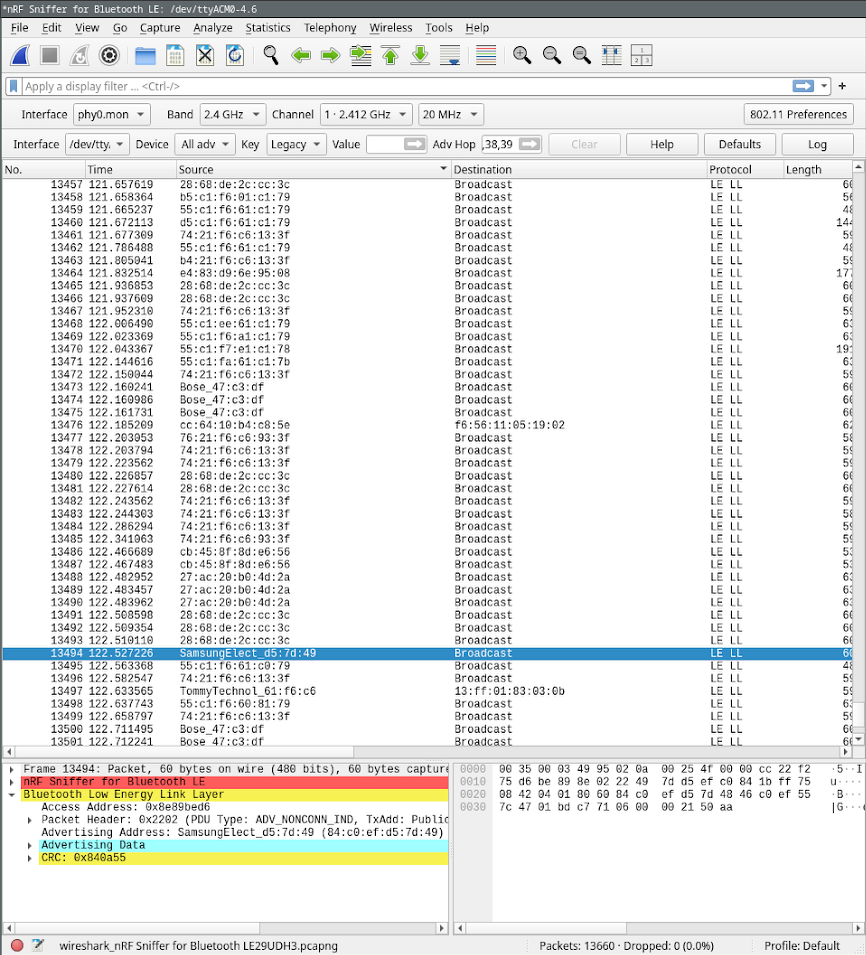
\includegraphics[width=1.0\textwidth]{assets/ble_noise.png}
	\caption{Caption for the figure.}
	\label{fig:test_figure}
\end{figure}

Here is a citation \parencite{bluetooth-history-wiki}.
The bibliography is printed with the ``printbibliography" keyword below.

\printbibliography

\end{document}
